\section*{communication}
Unlike most servo motors Dynamixel uses digital packet communication instead of pulse-width modulation (PWM) signals.
By grouping data into different packages and transmitting it as a bundle.
This in turn opens up for many possibilities since the motors responds to commands,
have built in control functions together with memory allocation on the motor itself.
Dynamixel recommends two different setups for communication,
either by using a Tri-state-buffer to construct your own communication bridge  based on Universal asynchronous receiver-transmitter setup (UART). Or by using their own solution called U2D2.
In essense, the U2D2 uses the same protocol but also enables for USB communication between the controller and Dynamixels\cite{robotis}.

\subsection{UART full duplex to half duplex}
UART communication scheme works by connecting the transmitter pin (Tx) of the Jetson Nvidia Nano microcontroller (MCU)
directly to the receiver pin (Rx) of the motors and vice versa.
UART communication can be setup into three different ways of communication \cite{duplex}.
Full duplex, half duplex and simplex.
Full duplex allows for data communication both ways simultaneously.
Half duplex only allows for one way communication at any given time, by either sending or receiving.
Simplex communication is static, meaning communication happens in one direction.
\newline
Full duplex and half duplex are not directly compatible. 
If the MCU and Dynamixel motors are connected directly,
since the MCU sends and receive data simultaneously it will occupy the transmission line indefinitely and the Dynamixel won't be able to tell when the messages stop. 
This phenomena is known as chatter. 
The solution for this is to implement a tri-state-buffer circuit converting the full system to half duplex.

\subsection{Tri-state-buffer}

A tri-state-buffer dictates when the MCU is allowed to communicate with the motors. This explained  by figure \ref{duplex}.
By controlling the direction pin (GPIO pin),
we can direct the flow of data. 
If the direction pin is pulled high we simultaneously allow for transmission from the MCU (Tx) to the motors and disable the MCU receiver pin (Rx).
A crucial part is timing, the direction pin must be pulled high long enough for the data to transfer through the buffer otherwise information is lost.
A logic analyzer will give this information and is recommended to use in conjugation with the tri-state-buffer for tuning.

\subsection{Data package - structure of message}
The protocol allows for a size of 8 bits per message between the MCU and motors. 
The two types message structures is represented by the figures below \ref{instr} and \ref{return}.
For more information how to interpret the structure use dynamixels own documentation ().

\subsubsection{Instruction package}
Instruction package carries commands from the controller to the motor.
An abundance of support is included,
from changing statics parameters like torque, baud-rate or id of each individual unit or different actions,
for example move to this location with this speed.
The structure of the message is represented in figure \ref{instr} and table \ref{instr_table} describes the structure from left to right. 

\begin{table}[H]
    \centering
    \caption{Explanation of parameters in instruction packadge}
    \begin{tabular}{c | c c c c c}
        \(OXFF\) & Indicates start of incoming packet  \\
        \hline
        \(ID\) & Specific ID of each unit  \\
        \hline
        \(Length\) & Length of message \\
        \hline
        \(Param\) & Used for additional information  \\
        \hline
        \(Check sum\) & Calculate length of packet \\
        \hline
    \end{tabular}
    \label{instr_table}
\end{table}

\begin{figure}[H]
    \graphicspath{ {img/} }
    \centering
    
    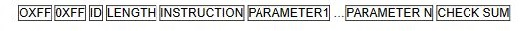
\includegraphics[width = 9 cm]{img/instruction_packadge}
    \label{instr}
    \caption{Structure of instruction message.}
\end{figure}

\subsubsection{Status package}
Status packet contains the response from the Dynamixel to the controller after receiving a instruction.
The structure is almost the same as the instruction package.
However, one difference is the the message confirms the status of sent instructions including an error if one occurs.
The structure is represented in figure \ref{return} and Dynamixels support page \cite{protocol1} gives more information how to read the error messages.

\begin{figure}[H]
    \graphicspath{ {img/} }
    \centering
    
    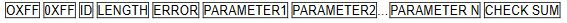
\includegraphics[width = 9 cm]{img/return_packadge.JPG}
    \label{return}
    \caption{Structure of return message.}
\end{figure}

\subsection{Motor communication}
Dynamixel provides a lot of support for lower level programming using instructions and reading return messages with documentation support, as stated above
. However, there is also support for higher level and more user friendly programming languages like Python,
C and third-party libraries by using Dynamixels own software development kit called DYNAMIXEL SDK \cite{dynamixel_SDK}.


